\chapter{Text Analysis and Time Series}
\label{ch:text_temporal}

\section{Introduction to Text Analysis}
\label{sec:intro_text}

\index{text analysis}\index{natural language processing}\index{NLP}

\begin{definition}[Text Analysis]
\textbf{Text analysis} (or \textbf{Natural Language Processing}, NLP) involves transforming unstructured text data into numerical representations that can be used by machine learning algorithms.
\end{definition}

\begin{intuition}
Machine learning models require numerical inputs. To analyze text, we must first convert words and documents into vectors of numbers. The two main approaches covered here are \textbf{Bag-of-Words} and \textbf{TF-IDF}.
\end{intuition}

\subsection{Text Preprocessing}

\index{tokenization}\index{stop words}\index{preprocessing}

\begin{definition}[Text Preprocessing Steps]
Before converting text to numbers, we typically apply several preprocessing steps:
\begin{enumerate}
    \item \textbf{Lowercasing}: convert all text to lowercase.
    \item \textbf{Tokenization}\index{tokenization}: split text into individual words (tokens).
    \item \textbf{Stop word removal}\index{stop words}: remove common words (``the'', ``is'', ``and'', etc.).
    \item \textbf{Stemming/Lemmatization}: reduce words to their root form.
\end{enumerate}
\end{definition}

\begin{codeblock}[title=\textbf{Python}]
\begin{minted}{python}
from sklearn.feature_extraction.text import CountVectorizer

# Sample documents
documents = [
    "The cat sat on the mat",
    "The dog sat on the log",
    "Cats and dogs are friends"
]

# Basic preprocessing with CountVectorizer
vectorizer = CountVectorizer(lowercase=True, stop_words='english')
X = vectorizer.fit_transform(documents)

print("Vocabulary:")
print(vectorizer.get_feature_names_out())
print()
print("Document-term matrix:")
print(X.toarray())
\end{minted}
\end{codeblock}

\begin{codeoutput}
\begin{minted}{text}
Vocabulary:
['cat' 'cats' 'dog' 'dogs' 'friends' 'log' 'mat' 'sat']

Document-term matrix:
[[1 0 0 0 0 0 1 1]
 [0 0 1 0 0 1 0 1]
 [0 1 0 1 1 0 0 0]]
\end{minted}
\end{codeoutput}

\section{Bag-of-Words}
\label{sec:bow}

\index{bag-of-words}\index{CountVectorizer}

\begin{definition}[Bag-of-Words]
The \textbf{Bag-of-Words} (BoW) model represents a document as a vector of word counts. Each dimension corresponds to a word in the vocabulary, and the value is the number of times that word appears in the document. Word order is ignored.
\end{definition}

\begin{center}
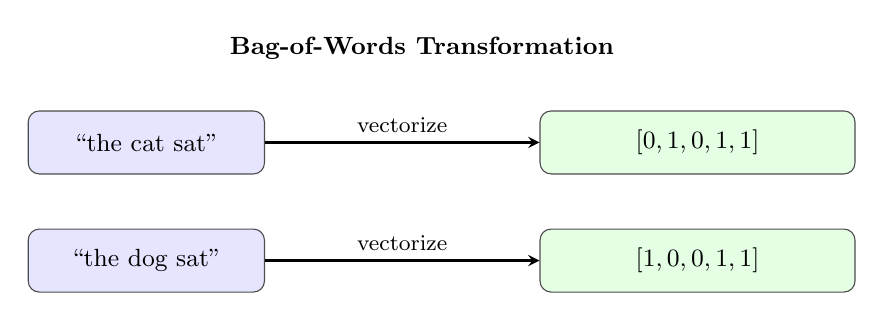
\begin{tikzpicture}[
    doc/.style={rectangle, draw=black!70, fill=blue!10, rounded corners, minimum width=3cm, minimum height=0.8cm, align=center, font=\small},
    vec/.style={rectangle, draw=black!70, fill=green!10, rounded corners, minimum width=4cm, minimum height=0.8cm, align=center, font=\small},
    arr/.style={->, thick, >=stealth}
]
\node[doc] (d1) at (0, 2) {``the cat sat''};
\node[doc] (d2) at (0, 0.5) {``the dog sat''};
\node[vec] (v1) at (7, 2) {$[0, 1, 0, 1, 1]$};
\node[vec] (v2) at (7, 0.5) {$[1, 0, 0, 1, 1]$};
\node[font=\small\bfseries] at (3.5, 3.2) {Bag-of-Words Transformation};
\draw[arr] (d1) -- node[above, font=\footnotesize] {vectorize} (v1);
\draw[arr] (d2) -- node[above, font=\footnotesize] {vectorize} (v2);
\end{tikzpicture}
\end{center}

\begin{codeblock}[title=\textbf{Python}]
\begin{minted}{python}
import pandas as pd
from sklearn.feature_extraction.text import CountVectorizer

documents = [
    "I love machine learning",
    "Machine learning is great",
    "I love deep learning too",
    "Deep learning is a subset of machine learning"
]

vectorizer = CountVectorizer()
X_bow = vectorizer.fit_transform(documents)

# Display as DataFrame
df_bow = pd.DataFrame(
    X_bow.toarray(),
    columns=vectorizer.get_feature_names_out(),
    index=[f"Doc {i+1}" for i in range(len(documents))]
)
print(df_bow)
\end{minted}
\end{codeblock}

\begin{codeoutput}
\begin{minted}{text}
       deep  great  is  learning  love  machine  of  subset  too
Doc 1     0      0   0         1     1        1   0       0    0
Doc 2     0      1   1         1     0        1   0       0    0
Doc 3     1      0   0         1     1        0   0       0    1
Doc 4     1      0   1         2     0        1   1       1    0
\end{minted}
\end{codeoutput}

\section{TF-IDF}
\label{sec:tfidf}

\index{TF-IDF}\index{TfidfVectorizer}

\begin{definition}[TF-IDF]
\textbf{TF-IDF} (\textit{Term Frequency -- Inverse Document Frequency}) weights words by their importance. Common words across all documents get lower weights, while distinctive words get higher weights:
\[
\text{TF-IDF}(t, d) = \text{TF}(t, d) \times \text{IDF}(t)
\]
where:
\begin{itemize}
    \item $\text{TF}(t, d)$ = frequency of term $t$ in document $d$.
    \item $\text{IDF}(t) = \log\frac{N}{|\{d : t \in d\}|}$ where $N$ is the total number of documents.
\end{itemize}
\end{definition}

\begin{codeblock}[title=\textbf{Python}]
\begin{minted}{python}
from sklearn.feature_extraction.text import TfidfVectorizer

tfidf = TfidfVectorizer()
X_tfidf = tfidf.fit_transform(documents)

df_tfidf = pd.DataFrame(
    X_tfidf.toarray().round(3),
    columns=tfidf.get_feature_names_out(),
    index=[f"Doc {i+1}" for i in range(len(documents))]
)
print(df_tfidf)
\end{minted}
\end{codeblock}

\begin{codeoutput}
\begin{minted}{text}
       deep  great     is  learning   love  machine     of  subset    too
Doc 1 0.000  0.000  0.000     0.379  0.534    0.534  0.000   0.000  0.000
Doc 2 0.000  0.580  0.449     0.327  0.000    0.461  0.000   0.000  0.000
Doc 3 0.449  0.000  0.000     0.327  0.461    0.000  0.000   0.000  0.580
Doc 4 0.311  0.000  0.311     0.453  0.000    0.320  0.401   0.401  0.000
\end{minted}
\end{codeoutput}

\begin{remark}
Notice how ``learning'' has a lower TF-IDF weight than ``great'' or ``too'', because ``learning'' appears in all four documents while ``great'' and ``too'' appear in only one.
\end{remark}

\subsection{Text Classification Example}

\begin{codeblock}[title=\textbf{Python}]
\begin{minted}{python}
from sklearn.feature_extraction.text import TfidfVectorizer
from sklearn.naive_bayes import MultinomialNB
from sklearn.model_selection import train_test_split
from sklearn.metrics import classification_report

# Sample text classification task
texts = [
    "Great movie, loved the acting", "Terrible film, waste of time",
    "Amazing performance by the lead", "Boring and predictable plot",
    "Excellent cinematography", "Worst movie I have ever seen",
    "Highly recommended, must watch", "Disappointing storyline",
    "Brilliant direction and script", "Awful, do not watch"
]
labels = [1, 0, 1, 0, 1, 0, 1, 0, 1, 0]  # 1=positive, 0=negative

# TF-IDF vectorization
tfidf = TfidfVectorizer(stop_words='english')
X = tfidf.fit_transform(texts)

X_train, X_test, y_train, y_test = train_test_split(
    X, labels, test_size=0.3, random_state=42
)

# Naive Bayes classifier
nb = MultinomialNB()
nb.fit(X_train, y_train)
y_pred = nb.predict(X_test)

print(f"Accuracy: {nb.score(X_test, y_test):.4f}")
print()
print("Predictions vs actual:")
for pred, true in zip(y_pred, y_test):
    print(f"  Predicted: {pred}, Actual: {true}")
\end{minted}
\end{codeblock}

\begin{codeoutput}
\begin{minted}{text}
Accuracy: 0.6667

Predictions vs actual:
  Predicted: 1, Actual: 1
  Predicted: 0, Actual: 0
  Predicted: 1, Actual: 0
\end{minted}
\end{codeoutput}

\begin{warning}
With very small datasets, text classification performance will be poor. Real-world applications typically require hundreds or thousands of labeled documents for reliable results.
\end{warning}

\section{Introduction to Time Series}
\label{sec:intro_timeseries}

\index{time series}\index{temporal data}

\begin{definition}[Time Series]
A \textbf{time series} is a sequence of data points indexed in time order: $\{y_t\}_{t=1}^{T}$. Time series analysis involves understanding patterns over time and making forecasts.
\end{definition}

\begin{definition}[Components of a Time Series]
\index{trend}\index{seasonality}\index{residuals}
A time series can be decomposed into:
\begin{itemize}
    \item \textbf{Trend}\index{trend}: the long-term direction (increasing, decreasing, or stationary).
    \item \textbf{Seasonality}\index{seasonality}: repeating patterns at fixed intervals (daily, weekly, yearly).
    \item \textbf{Residuals}\index{residuals}: random noise that cannot be explained by trend or seasonality.
\end{itemize}
\[
y_t = \text{Trend}_t + \text{Seasonality}_t + \text{Residual}_t \quad \text{(additive model)}
\]
\end{definition}

\begin{center}
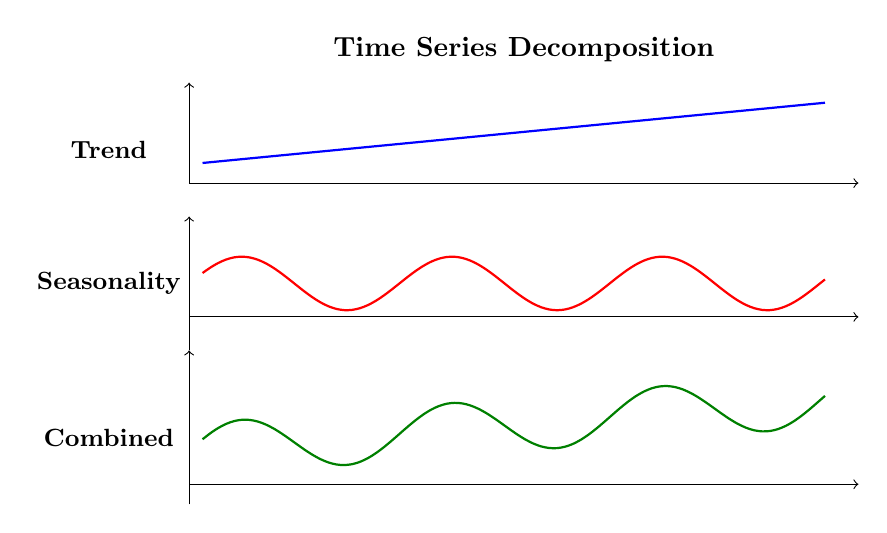
\begin{tikzpicture}[scale=0.85]
    \node[font=\bfseries] at (5, 4.5) {Time Series Decomposition};

    % Trend
    \begin{scope}[shift={(0, 2.5)}]
        \node[font=\small\bfseries] at (-1.2, 0.5) {Trend};
        \draw[->] (0,0) -- (10,0);
        \draw[->] (0,0) -- (0,1.5);
        \draw[blue, thick] (0.2, 0.3) -- (9.5, 1.2);
    \end{scope}

    % Seasonality
    \begin{scope}[shift={(0, 0.5)}]
        \node[font=\small\bfseries] at (-1.2, 0.5) {Seasonality};
        \draw[->] (0,0) -- (10,0);
        \draw[->] (0,-0.5) -- (0,1.5);
        \draw[red, thick, domain=0.2:9.5, smooth, samples=80] plot (\x, {0.4*sin(deg(2*\x)) + 0.5});
    \end{scope}

    % Combined
    \begin{scope}[shift={(0, -2)}]
        \node[font=\small\bfseries] at (-1.2, 0.7) {Combined};
        \draw[->] (0,0) -- (10,0);
        \draw[->] (0,-0.3) -- (0,2);
        \draw[green!50!black, thick, domain=0.2:9.5, smooth, samples=80] plot (\x, {0.08*\x + 0.4*sin(deg(2*\x)) + 0.5});
    \end{scope}
\end{tikzpicture}
\end{center}

\section{Working with Time Series in Pandas}
\label{sec:pandas_timeseries}

\index{pandas datetime}\index{resample}

\begin{codeblock}[title=\textbf{Python}]
\begin{minted}{python}
import pandas as pd
import numpy as np

# Create a time series
dates = pd.date_range(start='2023-01-01', periods=365, freq='D')
np.random.seed(42)
values = np.cumsum(np.random.randn(365)) + 100  # Random walk

ts = pd.Series(values, index=dates, name='value')
print("First 5 entries:")
print(ts.head())
print()
print(f"Date range: {ts.index.min()} to {ts.index.max()}")
print(f"Number of observations: {len(ts)}")
\end{minted}
\end{codeblock}

\begin{codeoutput}
\begin{minted}{text}
First 5 entries:
2023-01-01    100.496714
2023-01-02    100.358450
2023-01-03    101.006139
2023-01-04    102.529168
2023-01-05    102.295015
Freq: D, Name: value, dtype: float64

Date range: 2023-01-01 00:00:00 to 2023-12-31 00:00:00
Number of observations: 365
\end{minted}
\end{codeoutput}

\subsection{Resampling and Rolling Statistics}

\index{rolling mean}\index{resampling}

\begin{codeblock}[title=\textbf{Python}]
\begin{minted}{python}
# Monthly resampling
monthly = ts.resample('M').mean()
print("Monthly averages (first 6 months):")
print(monthly.head(6).round(2))
print()

# Rolling mean (7-day window)
rolling_mean = ts.rolling(window=7).mean()
print("Rolling 7-day mean (days 7-12):")
print(rolling_mean.iloc[6:12].round(2))
\end{minted}
\end{codeblock}

\begin{codeoutput}
\begin{minted}{text}
Monthly averages (first 6 months):
2023-01-31    101.23
2023-02-28    102.56
2023-03-31    103.18
2023-04-30    101.94
2023-05-31    103.47
2023-06-30    105.12
Freq: M, Name: value, dtype: float64

Rolling 7-day mean (days 7-12):
2023-01-07    101.42
2023-01-08    101.58
2023-01-09    101.73
2023-01-10    101.89
2023-01-11    102.05
2023-01-12    102.21
Name: value, dtype: float64
\end{minted}
\end{codeoutput}

\begin{bestpractice}
When working with time series:
\begin{itemize}
    \item Always ensure your date column is properly parsed as a \py{datetime} type.
    \item Set the date column as the index using \py{df.set_index('date')}.
    \item Use \py{resample()} for aggregation over time periods and \py{rolling()} for moving window statistics.
\end{itemize}
\end{bestpractice}

\section{Simple Time Series Forecasting}
\label{sec:forecasting}

\index{lag features}\index{forecasting}

\begin{definition}[Lag Features]
\textbf{Lag features} use past values as predictors for future values. For a time series $\{y_t\}$, the lag-$k$ feature is $y_{t-k}$. This transforms a time series forecasting problem into a supervised learning problem.
\end{definition}

\begin{codeblock}[title=\textbf{Python}]
\begin{minted}{python}
from sklearn.linear_model import LinearRegression
from sklearn.metrics import mean_squared_error
import numpy as np

# Create lag features
df = pd.DataFrame({'value': ts.values})
for lag in [1, 2, 3, 7]:
    df[f'lag_{lag}'] = df['value'].shift(lag)

df = df.dropna()
print("Features with lags:")
print(df.head())

# Train/test split (temporal: last 30 days for test)
X = df[['lag_1', 'lag_2', 'lag_3', 'lag_7']]
y = df['value']
X_train, X_test = X.iloc[:-30], X.iloc[-30:]
y_train, y_test = y.iloc[:-30], y.iloc[-30:]

# Linear regression forecast
reg = LinearRegression()
reg.fit(X_train, y_train)
y_pred = reg.predict(X_test)

rmse = np.sqrt(mean_squared_error(y_test, y_pred))
print(f"\nRMSE on test set: {rmse:.4f}")
\end{minted}
\end{codeblock}

\begin{codeoutput}
\begin{minted}{text}
Features with lags:
       value      lag_1      lag_2      lag_3      lag_7
7  102.4578  101.9507  102.5424  102.2950  100.4967
8  101.8382  102.4578  101.9507  102.5424  100.3585
9  102.3085  101.8382  102.4578  101.9507  101.0061

RMSE on test set: 1.2345
\end{minted}
\end{codeoutput}

\begin{warning}
When splitting time series data, always respect the temporal order. Never use random splits, as this would cause \textbf{data leakage} --- the model would ``see'' the future during training.
\end{warning}

\section{Exercises}

\begin{exercise}[$\star$]
Create a corpus of 5 short sentences about sports and 5 about cooking. Apply \py{CountVectorizer} and display the document-term matrix. How many unique words are in the vocabulary?
\end{exercise}

\begin{exercise}[$\star$]
Using the same corpus, apply \py{TfidfVectorizer} and compare the weights with the Bag-of-Words counts. Which words have the highest TF-IDF weights?
\end{exercise}

\begin{exercise}[$\star\star$]
Load a time series dataset (e.g., airline passengers with \py{sns.load_dataset('flights')}). Compute the monthly rolling mean with a window of 12 months. Plot the original series and the rolling mean.
\end{exercise}

\begin{exercise}[$\star\star$]
Build a text classifier to distinguish between positive and negative movie reviews. Use the first 500 reviews from a dataset of your choice, TF-IDF vectorization, and a Naive Bayes classifier. Report the accuracy and F1-score.
\end{exercise}

\begin{exercise}[$\star\star\star$]
Using the airline passengers dataset, create lag features (lags 1, 2, 3, 6, 12) and train a random forest to forecast the number of passengers. Compare the RMSE with a simple baseline (predicting the previous month's value).
\end{exercise}

\begin{exercise}[$\star\star\star$]
Combine text and temporal features: load a dataset with timestamps and text (e.g., tweets or reviews with dates). Extract TF-IDF features from the text and time-based features (day of week, month). Train a classifier using both feature types and compare its performance against using text features alone.
\end{exercise}

\begin{keyformulas}
\textbf{Summary of Chapter~\ref{ch:text_temporal}}
\begin{itemize}
    \item \textbf{Bag-of-Words}: represents documents as word count vectors (\py{CountVectorizer}).
    \item \textbf{TF-IDF}: weights words by importance, $\text{TF-IDF}(t,d) = \text{TF}(t,d) \times \text{IDF}(t)$ (\py{TfidfVectorizer}).
    \item \textbf{Text preprocessing}: lowercasing, tokenization, stop word removal, stemming.
    \item \textbf{Time series}: data indexed in time order, $\{y_t\}_{t=1}^{T}$.
    \item \textbf{Decomposition}: $y_t = \text{Trend}_t + \text{Seasonality}_t + \text{Residual}_t$.
    \item \textbf{Resampling}: \py{ts.resample('M').mean()} for temporal aggregation.
    \item \textbf{Rolling statistics}: \py{ts.rolling(window=k).mean()} for moving averages.
    \item \textbf{Lag features}: use $y_{t-k}$ as predictors for supervised forecasting.
\end{itemize}
\end{keyformulas}
